\documentclass{standalone}
\usepackage{tikz}
\usetikzlibrary{patterns, positioning}

\begin{document}
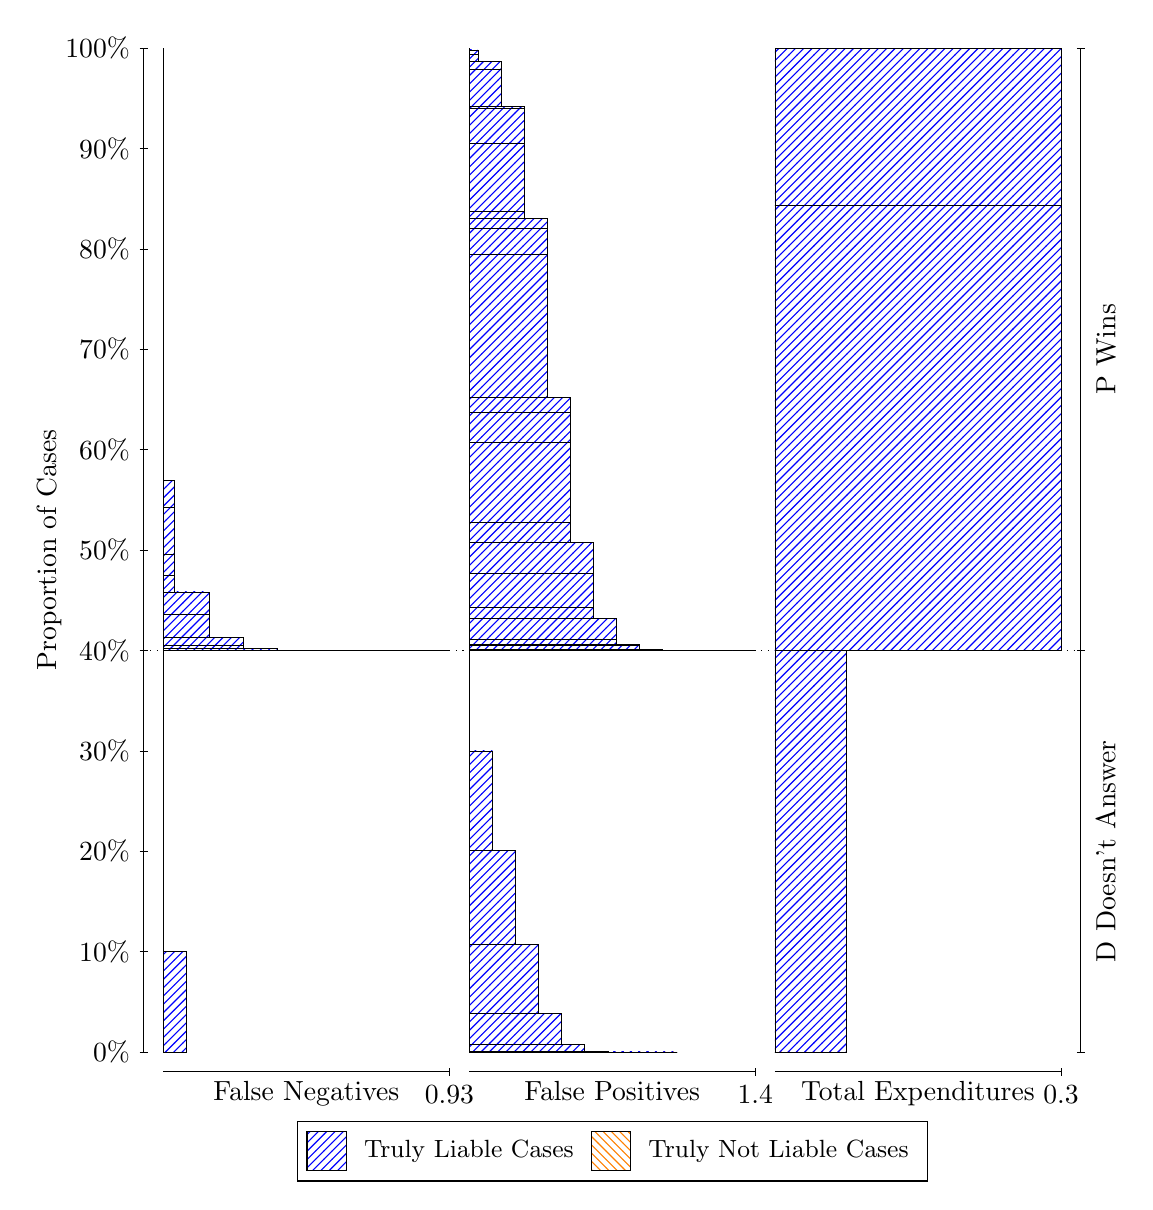
\begin{tikzpicture}
\draw[black, very thin] (1.5,1.75) -- (1.5,14.5);
\node[rotate=90, anchor=center] at (0.3, 8.125) {Proportion of Cases};
\draw[black, very thin] (1.45,1.75) -- (1.55,1.75);
\node[anchor=east] at (1.45, 1.75) {0\%};
\draw[black, very thin] (1.45,3.025) -- (1.55,3.025);
\node[anchor=east] at (1.45, 3.025) {10\%};
\draw[black, very thin] (1.45,4.3) -- (1.55,4.3);
\node[anchor=east] at (1.45, 4.3) {20\%};
\draw[black, very thin] (1.45,5.575) -- (1.55,5.575);
\node[anchor=east] at (1.45, 5.575) {30\%};
\draw[black, very thin] (1.45,6.85) -- (1.55,6.85);
\node[anchor=east] at (1.45, 6.85) {40\%};
\draw[black, very thin] (1.45,8.125) -- (1.55,8.125);
\node[anchor=east] at (1.45, 8.125) {50\%};
\draw[black, very thin] (1.45,9.4) -- (1.55,9.4);
\node[anchor=east] at (1.45, 9.4) {60\%};
\draw[black, very thin] (1.45,10.675) -- (1.55,10.675);
\node[anchor=east] at (1.45, 10.675) {70\%};
\draw[black, very thin] (1.45,11.95) -- (1.55,11.95);
\node[anchor=east] at (1.45, 11.95) {80\%};
\draw[black, very thin] (1.45,13.225) -- (1.55,13.225);
\node[anchor=east] at (1.45, 13.225) {90\%};
\draw[black, very thin] (1.45,14.5) -- (1.55,14.5);
\node[anchor=east] at (1.45, 14.5) {100\%};

\draw[black, very thin] (13.4,1.75) -- (13.4,14.5);
\draw[black, very thin] (13.35,1.75) -- (13.45,1.75);
\node[anchor=west] at (13.35, 1.75) {};
\draw[black, very thin] (13.35,6.8487) -- (13.45,6.8487);
\node[anchor=west] at (13.35, 6.8487) {};
\draw[black, very thin] (13.35,14.5) -- (13.45,14.5);
\node[anchor=west] at (13.35, 14.5) {};

\draw[black, very thin, pattern color=blue, pattern=north east lines] (1.75,1.75) rectangle (2.0446,3.0246);
\draw[black, very thin, pattern color=orange, pattern=north west lines] (1.75,3.0246) rectangle (1.75,3.0246);
\draw[black, very thin, pattern color=blue, pattern=north east lines] (1.75,3.0246) rectangle (1.75,6.8487);
\draw[black, very thin, pattern color=blue, pattern=north east lines] (1.75,6.8487) rectangle (5.3833,6.8487);
\draw[black, very thin, pattern color=blue, pattern=north east lines] (1.75,6.8487) rectangle (4.9469,6.8487);
\draw[black, very thin, pattern color=blue, pattern=north east lines] (1.75,6.8487) rectangle (4.5105,6.8487);
\draw[black, very thin, pattern color=blue, pattern=north east lines] (1.75,6.8487) rectangle (4.5105,6.8487);
\draw[black, very thin, pattern color=blue, pattern=north east lines] (1.75,6.8487) rectangle (4.074,6.8488);
\draw[black, very thin, pattern color=blue, pattern=north east lines] (1.75,6.8488) rectangle (3.6376,6.85);
\draw[black, very thin, pattern color=blue, pattern=north east lines] (1.75,6.85) rectangle (3.6376,6.8505);
\draw[black, very thin, pattern color=blue, pattern=north east lines] (1.75,6.8505) rectangle (3.2012,6.8723);
\draw[black, very thin, pattern color=blue, pattern=north east lines] (1.75,6.8723) rectangle (2.7647,6.9092);
\draw[black, very thin, pattern color=blue, pattern=north east lines] (1.75,6.9092) rectangle (2.7647,7.0185);
\draw[black, very thin, pattern color=blue, pattern=north east lines] (1.75,7.0185) rectangle (2.3283,7.3038);
\draw[black, very thin, pattern color=blue, pattern=north east lines] (1.75,7.3038) rectangle (2.3283,7.594);
\draw[black, very thin, pattern color=blue, pattern=north east lines] (1.75,7.594) rectangle (1.8918,7.7993);
\draw[black, very thin, pattern color=blue, pattern=north east lines] (1.75,7.7993) rectangle (1.8918,8.069);
\draw[black, very thin, pattern color=blue, pattern=north east lines] (1.75,8.069) rectangle (1.8918,8.6706);
\draw[black, very thin, pattern color=blue, pattern=north east lines] (1.75,8.6706) rectangle (1.8918,9.0076);
\draw[black, very thin, pattern color=orange, pattern=north west lines] (1.75,9.0076) rectangle (1.75,9.0076);
\draw[black, very thin, pattern color=blue, pattern=north east lines] (1.75,9.0076) rectangle (1.75,14.5);
\draw[black, very thin, pattern color=orange, pattern=north west lines] (5.6333,1.75) rectangle (8.2758,1.75);
\draw[black, very thin, pattern color=blue, pattern=north east lines] (5.6333,1.75) rectangle (8.2758,1.75);
\draw[black, very thin, pattern color=blue, pattern=north east lines] (5.6333,1.75) rectangle (7.9822,1.75);
\draw[black, very thin, pattern color=blue, pattern=north east lines] (5.6333,1.75) rectangle (7.6886,1.7503);
\draw[black, very thin, pattern color=blue, pattern=north east lines] (5.6333,1.7503) rectangle (7.3949,1.7582);
\draw[black, very thin, pattern color=blue, pattern=north east lines] (5.6333,1.7582) rectangle (7.1013,1.8434);
\draw[black, very thin, pattern color=blue, pattern=north east lines] (5.6333,1.8434) rectangle (6.8077,2.2368);
\draw[black, very thin, pattern color=blue, pattern=north east lines] (5.6333,2.2368) rectangle (6.5141,3.1183);
\draw[black, very thin, pattern color=blue, pattern=north east lines] (5.6333,3.1183) rectangle (6.2205,4.3076);
\draw[black, very thin, pattern color=blue, pattern=north east lines] (5.6333,4.3076) rectangle (5.9269,5.5741);
\draw[black, very thin, pattern color=blue, pattern=north east lines] (5.6333,5.5741) rectangle (5.6333,6.8487);
\draw[black, very thin, pattern color=orange, pattern=north west lines] (5.6333,6.8487) rectangle (9.2667,6.8487);
\draw[black, very thin, pattern color=blue, pattern=north east lines] (5.6333,6.8487) rectangle (9.2667,6.8487);
\draw[black, very thin, pattern color=orange, pattern=north west lines] (5.6333,6.8487) rectangle (8.9731,6.8487);
\draw[black, very thin, pattern color=blue, pattern=north east lines] (5.6333,6.8487) rectangle (8.9731,6.8487);
\draw[black, very thin, pattern color=orange, pattern=north west lines] (5.6333,6.8487) rectangle (8.6795,6.8487);
\draw[black, very thin, pattern color=blue, pattern=north east lines] (5.6333,6.8487) rectangle (8.6795,6.8488);
\draw[black, very thin, pattern color=blue, pattern=north east lines] (5.6333,6.8488) rectangle (8.3859,6.8489);
\draw[black, very thin, pattern color=orange, pattern=north west lines] (5.6333,6.8489) rectangle (8.3859,6.8489);
\draw[black, very thin, pattern color=blue, pattern=north east lines] (5.6333,6.8489) rectangle (8.3859,6.8495);
\draw[black, very thin, pattern color=orange, pattern=north west lines] (5.6333,6.8495) rectangle (8.0923,6.8495);
\draw[black, very thin, pattern color=blue, pattern=north east lines] (5.6333,6.8495) rectangle (8.0923,6.855);
\draw[black, very thin, pattern color=blue, pattern=north east lines] (5.6333,6.855) rectangle (8.0923,6.8566);
\draw[black, very thin, pattern color=blue, pattern=north east lines] (5.6333,6.8566) rectangle (8.0923,6.8585);
\draw[black, very thin, pattern color=orange, pattern=north west lines] (5.6333,6.8585) rectangle (7.7987,6.8585);
\draw[black, very thin, pattern color=blue, pattern=north east lines] (5.6333,6.8585) rectangle (7.7987,6.9168);
\draw[black, very thin, pattern color=blue, pattern=north east lines] (5.6333,6.9168) rectangle (7.7987,6.9282);
\draw[black, very thin, pattern color=blue, pattern=north east lines] (5.6333,6.9282) rectangle (7.5051,6.9941);
\draw[black, very thin, pattern color=orange, pattern=north west lines] (5.6333,6.9941) rectangle (7.5051,6.9941);
\draw[black, very thin, pattern color=blue, pattern=north east lines] (5.6333,6.9941) rectangle (7.5051,7.2558);
\draw[black, very thin, pattern color=blue, pattern=north east lines] (5.6333,7.2558) rectangle (7.2114,7.3977);
\draw[black, very thin, pattern color=orange, pattern=north west lines] (5.6333,7.3977) rectangle (7.2114,7.3977);
\draw[black, very thin, pattern color=blue, pattern=north east lines] (5.6333,7.3977) rectangle (7.2114,7.8243);
\draw[black, very thin, pattern color=blue, pattern=north east lines] (5.6333,7.8243) rectangle (7.2114,8.2223);
\draw[black, very thin, pattern color=blue, pattern=north east lines] (5.6333,8.2223) rectangle (6.9178,8.4756);
\draw[black, very thin, pattern color=orange, pattern=north west lines] (5.6333,8.4756) rectangle (6.9178,8.4756);
\draw[black, very thin, pattern color=blue, pattern=north east lines] (5.6333,8.4756) rectangle (6.9178,9.4909);
\draw[black, very thin, pattern color=blue, pattern=north east lines] (5.6333,9.4909) rectangle (6.9178,9.8758);
\draw[black, very thin, pattern color=blue, pattern=north east lines] (5.6333,9.8758) rectangle (6.9178,10.062);
\draw[black, very thin, pattern color=orange, pattern=north west lines] (5.6333,10.062) rectangle (6.6242,10.062);
\draw[black, very thin, pattern color=blue, pattern=north east lines] (5.6333,10.062) rectangle (6.6242,11.88);
\draw[black, very thin, pattern color=blue, pattern=north east lines] (5.6333,11.88) rectangle (6.6242,12.214);
\draw[black, very thin, pattern color=blue, pattern=north east lines] (5.6333,12.214) rectangle (6.6242,12.341);
\draw[black, very thin, pattern color=blue, pattern=north east lines] (5.6333,12.341) rectangle (6.3306,12.425);
\draw[black, very thin, pattern color=blue, pattern=north east lines] (5.6333,12.425) rectangle (6.3306,13.296);
\draw[black, very thin, pattern color=blue, pattern=north east lines] (5.6333,13.296) rectangle (6.3306,13.736);
\draw[black, very thin, pattern color=blue, pattern=north east lines] (5.6333,13.736) rectangle (6.3306,13.755);
\draw[black, very thin, pattern color=blue, pattern=north east lines] (5.6333,13.755) rectangle (6.037,14.231);
\draw[black, very thin, pattern color=blue, pattern=north east lines] (5.6333,14.231) rectangle (6.037,14.33);
\draw[black, very thin, pattern color=blue, pattern=north east lines] (5.6333,14.33) rectangle (5.7434,14.331);
\draw[black, very thin, pattern color=blue, pattern=north east lines] (5.6333,14.331) rectangle (5.7434,14.424);
\draw[black, very thin, pattern color=blue, pattern=north east lines] (5.6333,14.424) rectangle (5.7434,14.476);
\draw[black, very thin, pattern color=blue, pattern=north east lines] (5.6333,14.476) rectangle (5.7434,14.476);
\draw[black, very thin, pattern color=blue, pattern=north east lines] (5.6333,14.476) rectangle (5.6333,14.5);
\draw[black, very thin, pattern color=orange, pattern=north west lines] (9.5167,1.75) rectangle (10.425,1.75);
\draw[black, very thin, pattern color=blue, pattern=north east lines] (9.5167,1.75) rectangle (10.425,6.8487);
\draw[black, very thin, pattern color=orange, pattern=north west lines] (9.5167,6.8487) rectangle (13.15,6.8487);
\draw[black, very thin, pattern color=blue, pattern=north east lines] (9.5167,6.8487) rectangle (13.15,12.505);
\draw[black, very thin, pattern color=orange, pattern=north west lines] (9.5167,12.505) rectangle (13.15,12.505);
\draw[black, very thin, pattern color=blue, pattern=north east lines] (9.5167,12.505) rectangle (13.15,14.5);
\draw[black, dotted] (1.5,6.8487) -- (13.4,6.8487);
\draw[black, very thin] (1.75,1.5) -- (5.3833,1.5);
\node[anchor=north] at (3.5667, 1.5) {False Negatives};
\draw[black, very thin] (5.3833,1.45) -- (5.3833,1.55);
\node[anchor=north] at (5.3833, 1.45) {0.93};

\draw[black, very thin] (5.6333,1.5) -- (9.2667,1.5);
\node[anchor=north] at (7.45, 1.5) {False Positives};
\draw[black, very thin] (9.2667,1.45) -- (9.2667,1.55);
\node[anchor=north] at (9.2667, 1.45) {1.4};

\draw[black, very thin] (9.5167,1.5) -- (13.15,1.5);
\node[anchor=north] at (11.333, 1.5) {Total Expenditures};
\draw[black, very thin] (13.15,1.45) -- (13.15,1.55);
\node[anchor=north] at (13.15, 1.45) {0.3};

\node[black, centered, rotate=90] at (13.72, 4.2994) {D Doesn't Answer};
\node[black, centered, rotate=90] at (13.72, 10.674) {P Wins};

\draw (7.449999999999999,1.5) node[draw=none] (baseCoordinate) {};
\begin{scope}[align=center]
        \matrix[scale=0.5, draw=black, below=0.5cm of baseCoordinate, nodes={draw}, column sep=0.1cm]{
            \node[rectangle, draw, minimum width=0.5cm, minimum height=0.5cm, pattern=north east lines, pattern color=blue] {}; &
            \node[draw=none, font=\small] (B) {Truly Liable Cases}; &
            \node[rectangle, draw, minimum width=0.5cm, minimum height=0.5cm, pattern=north west lines, pattern color=orange] {}; &
            \node[draw=none, font=\small] (B) {Truly Not Liable Cases}; \\
            };
\end{scope}

\end{tikzpicture}
\end{document}